\begin{figure*}
\centering
\begin{subfigure}[h]{0.45\textwidth}
\caption{}
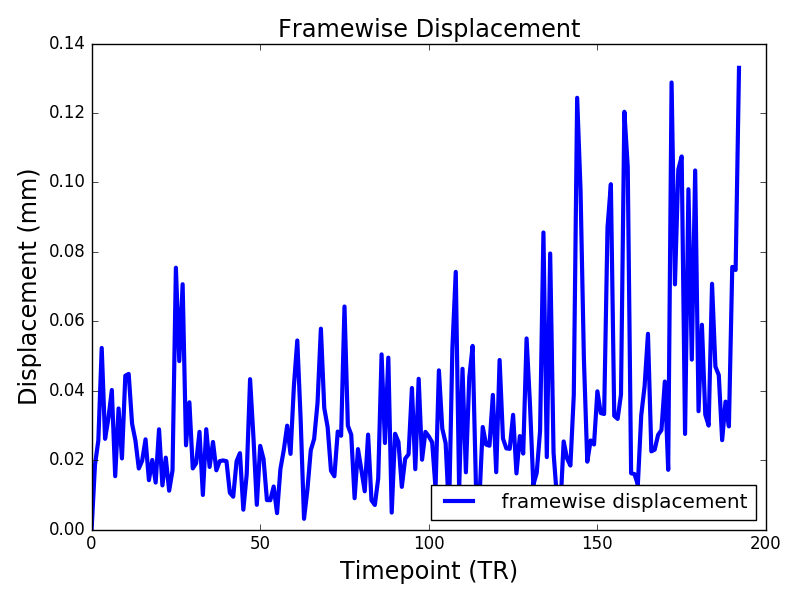
\includegraphics[width=\textwidth]{./qa_figs/fig_fmri_preproc.png}
\label{fig:fd}
\end{subfigure}
\begin{subfigure}[h]{0.45\textwidth}
\caption{}
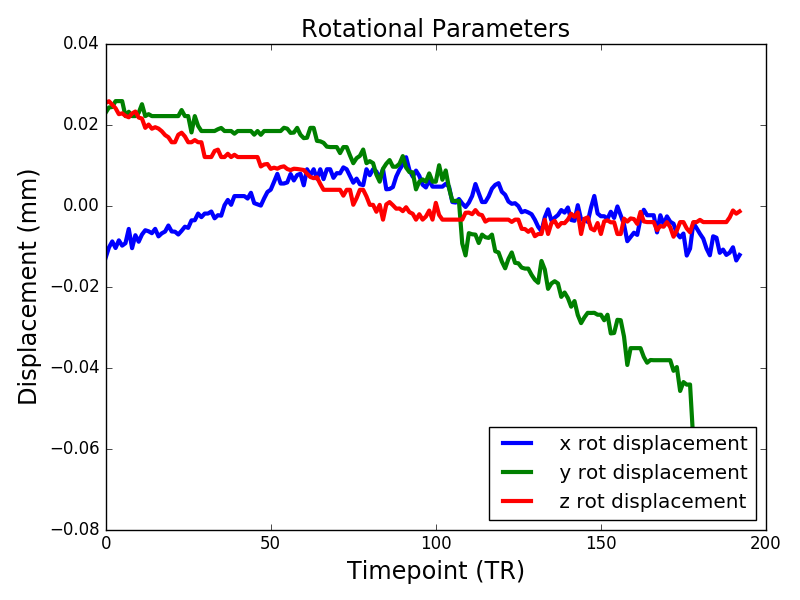
\includegraphics[width=\textwidth]{./qa_figs/fig_fmri_preproc_rot.png}
\label{fig:rot}
\end{subfigure}
\begin{subfigure}[h]{0.7\textwidth}
\caption{}
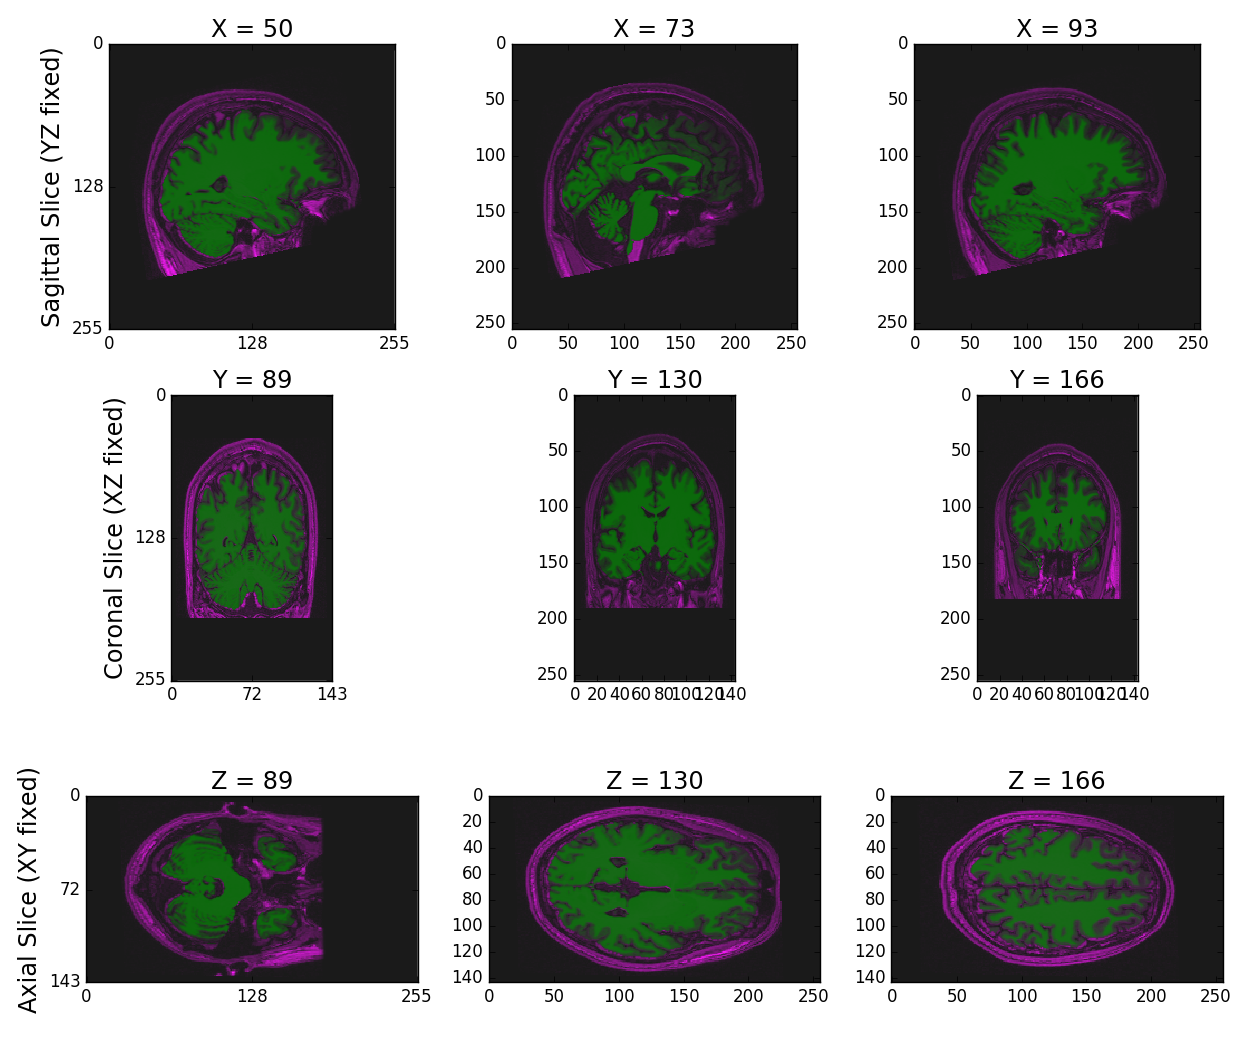
\includegraphics[width=\textwidth]{./qa_figs/fig_fmri_preproc_t1wbrain.png}
\label{fig:bet}
\end{subfigure}
\caption{\textbf{\ndmgf~Preprocessing QA}. For preprocessing, \ndmgf~produces QA figures showing (a) the framewise displacement per timestep, (b) the rotational and translational motion parameters, and (c) plots of the raw and corrected brain, and the success of the brain extraction process.}
% @reb: i don't understand what (c) is, please clarify.
% @rjv: (c) is just the motion-corrected average brain overlapped on the raw average brain. If motion is high, the average brain will be blurry, and motion cocrrection should show a less-blurred image.
% @eb: ok, explain which color is what, and the units on the X- and Y-axis.  if they are the same as a previous figure, define it in the previous figure, and then merely refer to them here.
\label{fig:fmri_preproc}
\end{figure*}